\documentclass[10pt,conference]{resources/IEEEtran}

%%% Start Preamble
\usepackage[T1]{fontenc}
\usepackage[utf8]{inputenc}
\usepackage[english]{babel}
\AtBeginDocument{%
	\providecommand\BibTeX{{%
			\normalfont B\kern-0.5em{\scshape i\kern-0.25em b}\kern-0.8em\TeX}}}

\usepackage{hyperref}
\usepackage{cite}

\usepackage{amsmath,amssymb,amsfonts} %amsmath already included
\usepackage[noend]{algpseudocode}
\usepackage{algorithmicx, algorithm}
\usepackage{graphicx} %graphicx already included
\usepackage{textcomp}
\usepackage{xcolor}

\usepackage{tikz}
\usetikzlibrary{arrows,decorations.markings, positioning}
\usepackage{subcaption}
\usepackage{tabu}

\hyphenation{con-straints}
%\pagestyle{plain}

%% COMMANDS:
\usepackage{resources/mathcommands}

%% DRAW SCHEDULES:
\usepackage{resources/scheduling}

%% THEOREMS:
% Theorems --
\usepackage{amsthm}

\newtheorem{thm}{Theorem}%[section]
\newtheorem{prop}[thm]{Proposition}
\newtheorem{lem}[thm]{Lemma}
\newtheorem{cor}[thm]{Corollary}
\newtheorem{obs}[thm]{Observation}

\theoremstyle{definition}
\newtheorem{defn}[thm]{Definition}
\newtheorem{notn}[thm]{Notation}

\theoremstyle{remark}
\newtheorem{rmk}[thm]{Remark}
\newtheorem{exmpl}[thm]{Example}
% --


%% WRITING:
\newcommand{\comment}[3]{{\color{#1}#2:#3}\ClassWarning{}{There are comments left in the paper. [Remove them before submission!]}}
\newcommand{\mario}[1]{\comment{red}{mg}{#1}}
\newcommand{\kuan}[1]{\comment{blue}{kh}{#1}}
\newcommand{\jj}[1]{\comment{orange}{jj}{#1}}

% \usepackage{lineno}
\usepackage[switch]{lineno}
\linenumbers
% fix problem with line numbering around align
\makeatletter
\let\LN@align\align
\let\LN@endalign\endalign
\renewcommand{\align}{\linenomath\LN@align}
\renewcommand{\endalign}{\LN@endalign\endlinenomath}
\makeatother


%% PAPER SPECIFIC:
\usetikzlibrary{patterns}

\newcommand{\mrt}{\mathrm{MRT}}
\newcommand{\lat}{\mathrm{Lat}}

\newcommand{\fc}{\fw{c}}
\newcommand{\bc}{\bw{c}}
\newcommand{\pc}{{pc}}

\newtheorem{lemma}{Lemma}
\theoremstyle{definition}
\newtheorem{definition}{Definition}
\newtheorem{theorem}{Theorem}
%\newtheorem{prog}[theorem]{Programming}
\newtheorem{prog}{Programming}



%%% End Preamble




\begin{document}
	%% TITLE:
	\title{Optimal Task Phasing for End-To-End Latency in Harmonic and Semi-Harmonic Automotive Systems}
	
	%% AUTHORS: Mario, Matthias
	
%	% Final version
%	\author{
%		\IEEEauthorblockN{First Author, Second Author and Third Author}
%		\IEEEauthorblockA{TU Dortmund University\\
%			Email: \{first.author, second.author, third.author\}@tu-dortmund.de}
%		\and
%		\IEEEauthorblockN{Other Author}
%		\IEEEauthorblockA{Other University\\
%			Email: other.author@other-university.de}
%		}
	
%	% Submission version:
	\author{RTAS 2025 Submission \# \textcolor{red}{TBD} \quad\quad\quad Pages: \pageref{last-page}}
	
	\maketitle

	\begin{abstract}
		% - introductory sentence to the topic (optional)
		In the context of automotive systems, the end-to-end latency of a sequence of tasks (a so-called cause-effect chains) is a common metric to ensure correct timing behavior.
		% - describe the issue or main problem (create a need)
		To control the end-to-end latency, proper task configuration is crucial. 
		While the literature considers the configuration of task periods, optimization of task phases to minimize the end-to-end latency is only sparsely discussed. 

		% - one sentence detailing your approach (meet the need)
		In this work, we discuss the configuration of task phases to optimize the end-to-end latency of a cause-effect chain.
		% - list main research results
		To that end, we develop a strategy for semi-harmonic task systems, which are very common in industrial applications.
		% - finish with MAIN MESSAGE of the paper
		We prove that our strategy is optimal in the sense that it minimizes the end-to-end latency.
		Furthermore, our evaluation based on a real-world application shows that optimizing task phases can reduce end-to-end latencies significantly. 

		\mario{11 pages of technical content + bib and ackn; Track 2}
	\end{abstract} 
	
%	\vspace{-.2in}
	
	\section{Introduction}
	\label{sec:introduction}
	% General introduction

	% Topic of this paper
	
	% Detailed topic / tell more details


	State of the art: Release all tasks at the same time


	- Related work: Alessandro ECRTS
	
	
	% Contribution
	\noindent\textbf{Contributions:} % short text
	\begin{itemize}
		\item one
		\item two
		\item three
	\end{itemize}
	
\section{System Model}
\label{sec:system_model}

	In embedded systems, several tasks are deployed that each fulfills a different dedicated purpose (Lidar, Location, EKF, Camera, etc. in Figure~\ref{fig:example}).
	The set of all tasks is denoted as $\Tbb$.
	%
	To allow the embedded system to fulfill complex assignments, tasks have to interact with each other. 
	That is achieved by data exchange between tasks. 
	More specifically, data is written to and read from shared resources. 
	In the case of the running example in Figure~\ref{fig:example}, the Lidar sensor writes its data to a shared register, where the data can be picked up by the Localization and the Planner algorithm.
	This communication behavior spans a graph of data dependencies visualized in Figure~\ref{fig:example}.
	Each path in this graph of data dependencies describes one cause-effect chain to be analyzed. 

	\textbf{Task Model:}
	Each task $\tau\in \Tbb$ can be described by a tuple $\tau=(C_\tau, T_\tau, \phi_\tau) \in \Rbb^3$.
	More specifically, $C_\tau >0$ is the worst-case execution time (WCET) of $\tau$, $T_\tau > 0$ is the task period, and $\phi_\tau$ is the task phase.
	The task recurrently releases jobs, denoted by $\tau(m),~m\in \Nbb {=} \setof{0,1,2,\dots}$ according to its description.
	That is, $\tau(0)$ is released at time $\phi_\tau$, and subsequent jobs are released every $T_{\tau}$ time units, i.e., $\tau(m)$ is released at time $\phi_\tau + m T_{\tau}$. 
	Each job $\tau(m)$ executes for at most $C_\tau$ time units.
	We consider implicit-deadline tasks where the deadline of each job is at the release of the subsequent job, i.e., the deadline of $\tau(m)$ is at $\phi_\tau + (m+1) T_{\tau}$.

	This work especially emphasizes the usage of \emph{harmonic} task systems, where all task periods are integer multiples of one another.
	That is, for any two tasks $\tau, \tau'$, we have $\frac{T_{\tau}}{T_{\tau'}} \in \Nbb$ or $\frac{T_{\tau'}}{T_{\tau}} \in \Nbb$.
	Harmonic task systems have the benefit that their release pattern is highly repetitive. As a result, the data propagation through these tasks is easier to analyze and to control.
	For the majority of analytical results, a weaker form of harmonic is already sufficient to obtain the results.
	That is, for any task $\tau \in \Tbb$, we have $\frac{\max_{\tau'\in \Tbb} T_{\tau'}}{T_{\tau}} \in \Nbb$.
	In this case we say that $\Tbb$ is \emph{semi-harmonic}.

	\textbf{Scheduling Model:}
	The jobs are scheduled utilizing a preemptive Rate-Monotonic (RM) scheduling. 
	That is, the priority of each task is given by the task period (the lower the period, the higher the priority) and at each point in time the highest priority pending task is executed. 
	For general (not harmonic) task sets, the utilization bound is $\ln(2)$~\cite{liu73scheduling}, i.e., if the total utilization $U=\sum_{\tau\in \Tbb} \frac{C_\tau}{T_\tau}$ is at most $\ln(2)$ then all jobs meet their deadline under RM scheduling.
	In the case that the task set is harmonic, the utilization bound is $1$~\cite{Liu:2000:RS:518501}.

	For the simplicity of presentation, this work focuses on uniprocessor systems, i.e., all tasks are scheduled on a single processsor.
	However, the results can easily be extended to any other scheduling mechanism and to synchronized multiprocessor systems by choosing the respective utilization bound from the literature~\cite{liu73scheduling,DBLP:journals/rts/LopezDG04,DBLP:conf/ecrts/AnderssonJ03,DBLP:conf/opodis/Andersson08,DBLP:conf/rtss/AnderssonBJ01,DBLP:journals/rts/OhB98,DBLP:conf/ecrts/LakshmananRL09,DBLP:conf/rtns/BruggenUCF17,DBLP:conf/rtas/GuanSYY10,DBLP:conf/sies/AnderssonT09}.
	As an example, if tasks are scheduled using partitioned RM scheduling, then the system is schedulable if the respective utilization bound on each processor $P$ is not exceeded, i.e.,
	\begin{math}
		% \max_{P \text{ processor}} 
		\sum_{\tau \text{ on } P} \frac{C_\tau}{T_\tau} < 1 
	\end{math}
	for harmonic tasks and 
	\begin{math}
		% \max_{P \text{ processor}} 
		\sum_{\tau \text{ on } P} \frac{C_\tau}{T_\tau} < \ln(2)
	\end{math}
	for the general case.

	\textbf{Data Dependency Graph:}
	Usually, functionalities are performed by several tasks.
	To achieve this, data has to be transmitted between tasks and the execution behavior of one task depends on the data obtained by the previous tasks. 
	This data dependency can be formalized using a directed acyclic graph (DAG).
	More specifically, each task forms one node of the DAG, and each data dependency corresponds to one edge in the DAG.
	Figure~\ref{fig:example} demonstrates the DAG structure of the data dependencies.
	Usually, there are timing constraints on different paths of the DAG.
	% \mario{Note that data dependency are not precedence constraints, i.e., task release jobs according to their period.}

	\textbf{Task communication:}
	To transmit data between tasks according to the dependency graph, tasks have to communicate. 
	We assume that the communication can be modeled via shared resources. 
	That is, a task writes data to a shared resource (overwriting previous data), and the successor tasks reads the data from that shared resource. 
	In this work, we focus on the communication model of the Logical Execution Time (LET)~\cite{DBLP:conf/birthday/KirschS12} mechanism, where each job reads data at its release and writes data at its deadline.
	More specifically, the read-event of $\tau(m)$ is at time 
	\begin{math}
		\re (\tau(m)) := \phi_{\tau} + m \cdot T_{\tau},
	\end{math}
	and the write-event of $\tau(m)$ is at time 
	\begin{math}
		\we (\tau(m)) := \phi_{\tau} + (m+1) \cdot T_{\tau}.
	\end{math}

	{We assume that the communication overheads are negligible, which can be realized by existing LET implementations~\cite{Biondi2018LET, Bellassai2023JSA7}.}
	Furthermore, we assume that each task $\tau \in \Tbb$ is part of a cause-effect chain. 
	However, this assumption is only for the sake of readability. 
	When a task is not part of a cause-effect chain, i.e., no timing requirement for that task is specified, its period and phase can either be fixed by the designer, or we minimize the utilization with $T_\tau \to \infty$.



\section{Cause-Effect Chains and End-to-End latencies}

	A specific path in the data dependency graph is called a cause-effect chain $E$.
	We denote a cause-effect chain by $E=(\tau_1 \to \dots \to \tau_n)$ for some $n\in \Nbb$.
%
	To ensure proper timely behavior of the system, each cause-effect chain is equipped with a timing requirement, i.e., an upper bound $B \in \Rbb>0$ on the \emph{end-to-end latency} along the cause-effect chain $E$.

	In the literature, two metrics for the end-to-end latency are usually considered:
	\begin{enumerate}
		\item Maximum Reaction Time: \emph{How long does it take until an external activity is processed?}
		\item Maximum Data Age: \emph{How old is data used in an actuation?}
	\end{enumerate}
	Recently, it was shown that both metrics are equivalent~\cite{DBLP:conf/ecrts/GunzelTCBC23}.
	Therefore, we do not distinguish those metrics and use the term \emph{end-to-end latency} ($\lat(E)$) universally.
	Further, it was shown in~\cite{DBLP:conf/ecrts/GunzelTCBC23} that \emph{partitioned job chains} can be used to define the end-to-end latency.
	Partitioned job chains rely on immediate forward and immediate backward job chains~\cite{duerrCASES}, which are used to track data propagation and data origin through the system, respectively.

	\begin{definition}[Immediate forward job chain]
		Let $m\in \Nbb$ and $E=(\tau_1\to \dots \to \tau_n)$ a cause-effect chain.
		The $m$-th \emph{immediate forward job chain} of $E$ is a sequence of jobs 
		\begin{math}
			\fc_m = (\tau_1(j_1) \to \dots \to \tau_n(j_n))
		\end{math}
		such that $j_1 = m$, and for all $i=1,\dots, n{-}1$ the job $\tau_{i+1}(j_{i+1})$ is the \emph{earliest} job of $\tau_{i+1}$ that reads data after it is written by $\tau_{i}(j_i)$, i.e., 
		\begin{math}
			j_{i+1} = \min \set{\xi \in \Nbb}{
			\we(\tau_i(j_i)) \leq 
			\re(\tau_{i+1}(\xi))
			}
			= \min \set{\xi \in \Nbb}{
			\phi_{\tau_i} + (j_i +1) \cdot T_{\tau_i} \leq 
			\phi_{\tau_{i+1}} + \xi \cdot T_{\tau_{i+1}}}.
		\end{math}
	\end{definition}

	\begin{definition}[Immediate backward job chain]
		Let $m\in \Nbb$ and $E=(\tau_1\to \dots \to \tau_n)$ a cause-effect chain.
		The $m$-th \emph{immediate backward job chain} of $E$ is a sequence of jobs 
		\begin{math}
			\bc_m = (\tau_1(j_1) \to \dots \to \tau_n(j_n))
		\end{math}
		such that $j_n = m$, and for all $i=2,\dots, n$ the job $\tau_{i-1}(j_{i-1})$ is the \emph{latest} job of $\tau_{i-1}$ that writes data before it is read by $\tau_{i}(j_i)$, i.e., 
		\begin{math}
			j_{i-1} 
			= \max \set{\xi \in \Nbb}{ 
			\we(\tau_{i-1}(\xi)) \leq \re(\tau_i(j_i))	
			}
			= \max \set{\xi \in \Nbb}{ \phi_{\tau_{i-1}} + (\xi+1) \cdot T_{\tau_{i-1}} \leq \phi_{\tau_i} + j_i \cdot T_{\tau_{i}}}.
		\end{math}
	\end{definition}

	We note that for some small $m$ the immediate backward job chain may not always exist in case $\set{\xi \in \Nbb}{ 
		\we(\tau_{i-1}(\xi)) \leq \re(\tau_i(j_i))	
		} = \emptyset$.
	Intuitively, this means that the job $\tau_{i}(j_i)$ has no data to process because task $\tau_{i-1}$ has not been executed yet.
	Such a scenario can only occur during the initial startup of the system.
	However, typical analyses are more interested in the system behavior during runtime when the system is already properly warmed up.
	We follow~\cite{DBLP:conf/ecrts/GunzelTCBC23} to determine the warm-up phase of each job.

	\begin{definition}[Warm-up]
		Consider the cause-effect chain $E=(\tau_1\to \dots \to \tau_n)$.
		Let $W_i\in \Nbb$, such that $\bc_W = (\tau_1(W_1) \to \dots \to \tau_n(W_n) )$ is the \emph{first} immediate backward job chain that exists. 
		We say that task $\tau_i$ is \emph{warmed up} with respect to $E$ at job $\tau_i(W_i)$.
	\end{definition}

	Intuitively, a task is warmed up with the first job that generates data that propagates to the end of the cause-effect chain without being overwritten.
	%
	In the following, we introduce partitioned job chains and properly define the end-to-end latency of $E$.

	\begin{definition}[Partitioned job chain.]
		Let $m\in \Nbb$, $E = (\tau_1\to\dots\to\tau_n)$, and  $p\in \setof{1, \dots, n}$.
		The $m$-th $p$-partitioned job chain of $E$ is a tuple
		\begin{equation}
			\pc^p_m = (\bc_m,\fc_{m+1})
		\end{equation}
		of an immediate backward and an immediate forward job chain.
		More specifically, $\bc_m$ is the $m$-th immediate backward job chain of $(\tau_1 \to \dots \to \tau_p)$, 
		and $\fc_{m+1}$ is the $(m+1)$-th immediate forward job chain of $(\tau_p \to \dots \to \tau_n)$.
	\end{definition}

	We note that the $\pc^p_m = (\bc_m,\fc_{m+1})$ exists if and only if its first entry $\bc_m$ exists.
	Hence, the $\pc^p_m$ exists for all $m\geq W_p$.
	%
	The length of $\pc^p_m = (\bc_m, \fc_{m+1})$ with $\bc_m = (\tau_1(j_1) \to\dots\to \tau_p(j_p))$ and $\fc_{m+1} = (\tau_p(j'_p) \to\dots\to \tau_n(j'_n))$ is defined as 
	\begin{align}
		\ell(\pc^p_m) 
		&:= 
		\we(\tau_n(j'_n)) - \re(\tau_1(j_1))
		\\&=
		(j'_n +1) \cdot T_{\tau_n} + \phi_{\tau_n} - (j_1 \cdot T_{\tau_1} + \phi_{\tau_1}).
	\end{align}
	% i.e., the distance between reading of the first job $\tau_1(j_1)$ and writing of the last job $\tau_n(j'_n)$.
	An example of a partitioned job chain is shown in Fig.~\ref{fig:chainExamples}.
	
	\begin{figure}
		\centering
		\footnotesize
		\begin{tikzpicture}[yscale=0.22, xscale=0.21]

			\begin{scope}[shift={(0,6)}] % task one
				\taskname{$\tau_1$}
				
				\timeline{0}{39}{}
				% no labelling
				
				% \releases{0,5,10}
				% \deadlines{5,10}
				
				\exec{0}{6}
				\exec[fill=red]{6}{12}
				\exec{12}{18}
				\exec{18}{24}
				\exec{24}{30}
				\exec{30}{36}
				\execopen{36}{38.5}
				
				% no suspension
			\end{scope}
			
			\begin{scope}[shift={(0,4.5)}] % task two
				\taskname{$\tau_2$}
				
				\timeline{0}{39}{}
				% \labelling{0}{13}{2}{0}
				
				% \releases{0}
				% \deadlines{12}
				
				\exec[pattern={north east lines}]{3}{7}
				\exec{7}{11}
				\exec{11}{15}
				\exec[fill=red]{15}{19}
				\exec[fill=blue]{19}{23}
				\exec{23}{27}
				\exec{27}{31}
				\exec{31}{35}
				\execopen{35}{38.5}

			\end{scope}

			\begin{scope}[shift={(0,3)}] % task three
				\taskname{$\tau_3$}
				
				\timeline{0}{39}{}
				% \labelling{0}{13}{2}{0}
				
				% \releases{0}
				% \deadlines{12}
				
				\exec[pattern={north east lines}]{0}{6}
				\exec[pattern={north east lines}]{6}{12}
				\exec{12}{18}
				\exec{18}{24}
				\exec[fill=blue]{24}{30}
				\exec{30}{36}
				\execopen{36}{38.5}

			\end{scope}

			\begin{scope}[shift={(0,1.5)}] % task four
				\taskname{$\tau_4$}
				
				\timeline{0}{39}{}
				\labelling{0}{39}{4}{0}
				
				% \releases{0}
				% \deadlines{12}
				
				\exec[pattern={north east lines}]{1}{5}
				\exec[pattern={north east lines}]{5}{9}
				\exec[pattern={north east lines}]{9}{13}
				\exec[pattern={north east lines}]{13}{17}
				\exec[pattern={north east lines}]{17}{21}
				\exec{21}{25}
				\exec{25}{29}
				\exec{29}{33}
				\exec[fill=blue]{33}{37}
				\execopen{37}{38.5}

			\end{scope}
		\end{tikzpicture}	
		\caption{A cause-effect chain $E=(\tau_1\rightarrow\tau_2\rightarrow\tau_3\rightarrow\tau_4)$ with LET communication semantics.  
			The partitioned job chain $\pc^2_4 = (\bc_4,\fc_5)$ is colorized. 
			The warm-up phase is indicated by jobs with hatched filling.} 
		\label{fig:chainExamples}
	\end{figure}

	\begin{definition}[End-to-end latency]
		The end-to-end latency of a cause-effect chain $E =(\tau_1\to\dots\to \tau_n)$ is the maximal length of $p$-partitioned job chains after the warm-up for any $p \in \setof{1, \dots, n}$.
		That is, 
		\begin{equation}
			\lat(E) = \sup_{m\geq W_p} \ell(\pc^p_m).
		\end{equation}		
	\end{definition}

	It is shown in~\cite{DBLP:conf/ecrts/GunzelTCBC23} that the end-to-end latency is independent of the choice of $p$, i.e., any $p \in \setof{1,\dots, n}$ can be chosen.



\section{Motivating Example}

	Show that releasing all jobs at the same time is not optimal, and that you can get better results by manipulating phases.
	
\section{Problem Definition}
\label{sec:problem_def}

	What is the best phasing? Nobody has looked into that yet. 

\section{Optimal Task Phasing for Harmonic Systems}


	Indeed, the results of this section work even for a larger class of task systems. 
	
	\begin{definition}[Max-Harmonic]
		A task system is called \emph{max-harmonic} if all periods divide the largest period, i.e., 
		\begin{equation}
			\frac{T_{\mathit{max}}}{T_{\tau_i}} \in \Nbb
		\end{equation}
		for all $\tau_i \in \Tbb$, where $T_{\mathit{max}} := \max_{\tau\in \Tbb} T_{\tau}$.
	\end{definition}

	\begin{lemma}[Optimality of task phasing]
		The end-to-end latency of $E$ under \emph{any} task phasing is lower bounded by $\sum_{i=1}^{n} T_{\tau_i} + \max_{i=1, \dots, n} T_{\tau_i}$.
		Hence, the task phasing from Theorem~\ref{thm:key} is optimal.
	\end{lemma}

	\begin{proof}
		Let $p\in \setof{1, \dots, n}$ such that $\tau_p$ is the task with the maximal period, i.e., $T_{\tau_p} = \max_{i=1, \dots, n} T_{\tau_i}$.
		Consider any $p$-partitioned job chain $\pc^p_m = (\bc_m,\fc_{m+1})$.
		We denote the immediate backward job chain by $\bc_m = (\tau_1(j_1) \to\dots\to \tau_p(j_p))$ and the immediate forward job chain by $\fc_{m+1} = (\tau_p(j'_p) \to\dots\to \tau_n(j'_n))$.
		%
		The length of $\pc^p_m$ can be expressed by:
		\begin{align}
			\ell(\pc^p_m) &= \we(\tau_n(j'_n)) - \re(\tau_1(j_1))
			\\& = \we(\tau_n(j'_n)) - \we(\tau_p(j'_p)) \label{eq:summand1}
			\\& \phantom{=} + \we(\tau_p(j'_p)) - \re(\tau_p(j_p)) \label{eq:summand2}
			\\& \phantom{=} + \re(\tau_p(j_p)) - \re(\tau_1(j_1)) \label{eq:summand3}
		\end{align}
		In the following we investigate each summand (Equations~\eqref{eq:summand1},~\eqref{eq:summand2},~\eqref{eq:summand3}) individually.

		\textbf{Summand of Equation~\eqref{eq:summand1}:}
		Equally, this summand can be written as the sum
		$\eqref{eq:summand1} = \sum_{i=p+1}^{n} (\we(\tau_i(j'_i)) - \we(\tau_{i-1}(j'_{i-1})))$.
		We use the property $\we(\tau_{i-1}(j'_{i-1})) \leq \re(\tau_i(j'_i))$ of immediate forward job chains to bound \eqref{eq:summand1} from below by 
		$\eqref{eq:summand1} \geq \sum_{i=p+1}^{n} (\we(\tau_i(j'_i)) - \re(\tau_{i}(j'_{i})))$.
		Since $\we(\tau_i(j'_i)) - \re(\tau_{i}(j'_{i})) = T_{\tau_i}$, we obtain $\eqref{eq:summand1} \geq \sum_{i=p+1}^{n} T_{\tau_i}$.

		\textbf{Summand of Equation~\eqref{eq:summand2}:}
		By definition, $j_p = m$ and $j'_p = m+1$.
		Therefore, $\eqref{eq:summand2} = (\phi_{\tau_p} + (m+1+1) \cdot T_{\tau_p}) - (\phi_{\tau_p} + m \cdot T_{\tau_p}) = 2\cdot T_{\tau_p}$.

		\textbf{Summand of Equation~\eqref{eq:summand3}:}
		This summand is
		$\eqref{eq:summand3} = \sum_{i=1}^{p-1} ( \re(\tau_{i+1}(j_{i+1})) - \re(\tau_i(j_i)) )$.
		We use the property $\re(\tau_{i+1}(j_{i+1})) \geq \we(\tau_i(j_i))$ of immediate backward job chains to achieve
		$\eqref{eq:summand3} \geq \sum_{i=1}^{p-1} ( \we(\tau_i(j_i)) - \re(\tau_i(j_i)) ) = \sum_{i=1}^{p-1} T_{\tau_i}$.

		We conclude $\ell(\pc^p_m) = \eqref{eq:summand1} + \eqref{eq:summand2} + \eqref{eq:summand3} \geq \sum_{i=1}^{n} T_{\tau_i} + T_{\tau_p} = \sum_{i=1}^{n} T_{\tau_i} + \max_{i=1, \dots, n} T_{\tau_i}$.
		Hence, $\lat(E) =\sup_{m\geq W_p} \ell(\pc^p_m) \geq \sum_{i=1}^{n} T_{\tau_i} + \max_{i=1, \dots, n} T_{\tau_i}$ under any task phasing.
		%
		Since the task phasing $\phi_{\tau_i} = \sum_{\xi=1}^{i-1} T_{\tau_\xi}$ achieves the minimal end-to-end latency, as stated in Theorem~\ref{thm:key}, this phasing is optimal.
	\end{proof}

	\begin{lemma}\label{lem:key_lemma}
		If $\setof{\tau_1, \dots, \tau_n}$ is semi-harmonic (in the sense as described in Section~\ref{sec:system_model}), then 
		\begin{equation}
			\ell(\pc^p_{W_p}) 
			= \ell(\pc^p_{W_p+1}) 
			= \ell(\pc^p_{W_p+2})
			= \dots 
		\end{equation}
		where $\tau_p$ is the task with the highest period, i.e., $T_{\tau_p} = \max_{i=1, \dots, n} T_{\tau_i}$.
	\end{lemma}

	\begin{proof}
		Let $m\geq W_p$.
		In the following we show that $\ell(\pc^p_{m}) 
		= \ell(\pc^p_{m+1})$.
	%
		By definition, $\pc^p_m = (\bc_m, \fc_{m+1})$ and $\pc^p_{m+1} = (\bc_{m+1}, \fc_{m+2})$.
		We start by investigating the immediate backward job chains, denoted as 
		$\bc_m = (\tau_1(j_1) \to\dots\to \tau_p(j_p))$ and $\bc_{m+1} = (\tau_1(\tilde{j}_1) \to\dots\to \tau_p({\tilde{j}}_p))$.
		By induction, we show that the jobs of both immediate backward job chains are exactly $T_{\tau_p}$ time units apart, or equivalently
		\begin{equation}\label{eq:induction1}
			j_i + \frac{T_{\tau_p}}{T_{\tau_i}} = \tilde{j}_i
		\end{equation}
		for all $i=p, p{-}1, \dots, 1$.

		\textbf{Base case} ($i=p$):
		By definition of the immediate backward job chains, $j_i = m $ and $\tilde{j}_i = m+1$.
		Hence, $j_i + \frac{T_{\tau_p}}{T_{\tau_i}} = m + \frac{T_{\tau_p}}{T_{\tau_p}} = m+1 = \tilde{j}_i$.

		\textbf{Induction step} ($i \mapsto i-1$):
		By definition of immediate backward job chains, 
		$j_{i-1} = \max \set{\xi \in \Nbb}{ \phi_{\tau_{i-1}} + (\xi+1) \cdot T_{\tau_{i-1}} \leq \phi_{\tau_i} + j_i \cdot T_{\tau_{i}}}$.
		Therefore, $j_{i-1}$ can be formulated as 
		$j_{i-1} = \floor{\frac{\phi_{\tau_i} - \phi_{\tau_{i-1}} + j_i \cdot T_{\tau_i}}{T_{\tau_{i-1}}}} -1$.
		Similarly, $\tilde{j}_{i-1}$ can be written as 
		$\tilde{j}_{i-1} = \floor{\frac{\phi_{\tau_i} - \phi_{\tau_{i-1}} + \tilde{j}_i \cdot T_{\tau_i}}{T_{\tau_{i-1}}}} -1$.
		We know by the induction hypothesis, that $\tilde{j}_i = j_i + \frac{T_{\tau_p}}{T_{\tau_i}}$.
		Therefore, 
		\begin{math}
			\tilde{j}_{i-1} 
			= \floor{\frac{\phi_{\tau_i} - \phi_{\tau_{i-1}} + j_i \cdot T_{\tau_i} + T_{\tau_p}}{T_{\tau_{i-1}}}} -1
			= \floor{\frac{\phi_{\tau_i} - \phi_{\tau_{i-1}} + j_i \cdot T_{\tau_i}}{T_{\tau_{i-1}}} + \frac{T_{\tau_p}}{T_{\tau_i}}} -1
			\overset{\text{(a)}}{=} \floor{\frac{\phi_{\tau_i} - \phi_{\tau_{i-1}} + j_i \cdot T_{\tau_i}}{T_{\tau_{i-1}}}} -1 + \frac{T_{\tau_p}}{T_{\tau_i}}
			= j_{i-1} + \frac{T_{\tau_p}}{T_{\tau_i}}
		\end{math}
		% \begin{align}
		% 	\tilde{j}_{i-1} 
		% 	&= \floor{\frac{\phi_{\tau_i} - \phi_{\tau_{i-1}} + j_i \cdot T_{\tau_i} + T_{\tau_p}}{T_{\tau_{i-1}}}} -1
		% 	= \floor{\frac{\phi_{\tau_i} - \phi_{\tau_{i-1}} + j_i \cdot T_{\tau_i}}{T_{\tau_{i-1}}} + \frac{T_{\tau_p}}{T_{\tau_i}}} -1
		% 	\\& \overset{\text{(a)}}{=} \floor{\frac{\phi_{\tau_i} - \phi_{\tau_{i-1}} + j_i \cdot T_{\tau_i}}{T_{\tau_{i-1}}}} -1 + \frac{T_{\tau_p}}{T_{\tau_i}}
		% 	= j_{i-1} + \frac{T_{\tau_p}}{T_{\tau_i}}
		% \end{align}
		where (a) holds because $\frac{T_{\tau_p}}{T_{\tau_i}} \in \Nbb$ by the semi-harmonic property. \qed~Equation~\eqref{eq:induction1}

		In the following we investigate the immediate forward chains, which we denote by
		$\fc_{m+1} = (\tau_p(j'_p) \to\dots\to \tau_n(j'_n))$ and $\fc_{m+2} = (\tau_p(\tilde{j}'_p) \to\dots\to \tau_n({\tilde{j}'}_n))$.
		We show that the jobs of both immediate forward job chains are also exactly $T_{\tau_p}$ time units apart.
		More specifically, we show by induction that 
		\begin{equation}\label{eq:induction2}
			j'_i + \frac{T_{\tau_p}}{T_{\tau_i}} = \tilde{j}'_i
		\end{equation}
		for all $i=p, p{+}1, \dots, n$.
		To achieve this, we additionally show that $j'_i, \tilde{j}'_i > W_i$ during the induction.

		\textbf{Base case} ($i=p$):
		By definition of the immediate forward job chains, $j'_i = m+1 $ and $\tilde{j}'_i = m+2$.
		Hence, $j'_i + \frac{T_{\tau_p}}{T_{\tau_i}} = m +1 + \frac{T_{\tau_p}}{T_{\tau_p}} = m+2 = \tilde{j}'_i$.
		Since $m \geq W_p$ by assumption, we obtain $j'_i = m+1 > W_i$ and $\tilde{j}'_i = m+2 > W_i$.

		\textbf{Induction step} ($i \mapsto i+1$):
		By definition of immediate forward job chains, 
		$j'_{i+1} = \min \set{\xi \in \Nbb}{\phi_{\tau_i} + (j'_i +1) \cdot T_{\tau_i} \leq \phi_{\tau_{i+1}} + \xi \cdot T_{\tau_{i+1}}}$.
		Therefore, $j'_{i+1}$ can be formulated as 
		$j'_{i+1} = \max\setof{\ceiling{\frac{\phi_{\tau_i} - \phi_{\tau_{i+1}} + (j'_i+1) \cdot T_{\tau_i}}{T_{\tau_{i+1}}}} , 0}$.
		
		We start by showing that $j'_{i+1}>W_{i+1}$ by contradiction.
		To that end, assume $j'_{i+1} \leq W_{i+1}$.
		Then, $\re(\tau_{i+1}(j'_{i+1})) \leq \re(\tau_{i+1}(W_{i+1}))$ as well.
		Since $\tau_i(j'_i)$ and $\tau_{i+1}(j'_{i+1})$ are two subsequent jobs in $\fc_{m+1}$, we have $\we(\tau_i(j'_i)) \leq \re(\tau_{i+1}(j'_{i+1}))$.
		Hence, $\we(\tau_i(j'_i)) \leq \re(\tau_{i+1}(W_{i+1}))$ holds.
		Since $W_i$ is the highest integer with $\we(\tau_i(W_i)) \leq \re(\tau_{i+1}(W_{i+1}))$, we obtain $W_i \geq j'_i$ which contradicts the induction hypothesis.

		Since we have shown that $j'_{i+1} > W_{i+1} \geq 0$, we know that $j'_{i+1}>0$.
		Hence, the maximum in $j'_{i+1} = \max\setof{\ceiling{\frac{\phi_{\tau_i} - \phi_{\tau_{i+1}} + (j'_i+1) \cdot T_{\tau_i}}{T_{\tau_{i+1}}}} , 0}$ always returns the first value. 
		That means that $j'_{i+1}$ can be formulated as
		\begin{math}
			j'_{i+1} = \ceiling{\frac{\phi_{\tau_i} - \phi_{\tau_{i+1}} + (j'_i+1) \cdot T_{\tau_i}}{T_{\tau_{i+1}}}}.
		\end{math}
		Similarly, we show that $\tilde{j}'_{i+1} > W_{i+1}$ and that 
		\begin{math}
			\tilde{j}'_{i+1} = \ceiling{\frac{\phi_{\tau_i} - \phi_{\tau_{i+1}} + (\tilde{j}'_i+1) \cdot T_{\tau_i}}{T_{\tau_{i+1}}}}.
		\end{math}
		%
		We utilize the induction hypothesis $\tilde{j}'_i = j'_i + \frac{T_{\tau_p}}{T_{\tau_i}}$ to obtain
		\begin{math}
			\tilde{j}'_{i+1} 
			= \ceiling{\frac{\phi_{\tau_i} - \phi_{\tau_{i+1}} + (j'_i +1) \cdot T_{\tau_i} + T_{\tau_p}}{T_{\tau_{i+1}}}}
			= \ceiling{\frac{\phi_{\tau_i} - \phi_{\tau_{i+1}} + (j'_i +1) \cdot T_{\tau_i}}{T_{\tau_{i+1}}} + \frac{T_{\tau_p}}{T_{\tau_{i+1}}}}
			= \ceiling{\frac{\phi_{\tau_i} - \phi_{\tau_{i+1}} + (j'_i +1) \cdot T_{\tau_i}}{T_{\tau_{i+1}}}} + \frac{T_{\tau_p}}{T_{\tau_{i+1}}}
			= j'_{i+1} + \frac{T_{\tau_p}}{T_{\tau_{i+1}}}
		\end{math}
		% \begin{align}
		% 	\tilde{j}'_{i+1} 
		% 	&= \ceiling{\frac{\phi_{\tau_i} - \phi_{\tau_{i+1}} + (j'_i +1) \cdot T_{\tau_i} + T_{\tau_p}}{T_{\tau_{i+1}}}}
		% 	= \ceiling{\frac{\phi_{\tau_i} - \phi_{\tau_{i+1}} + (j'_i +1) \cdot T_{\tau_i}}{T_{\tau_{i+1}}} + \frac{T_{\tau_p}}{T_{\tau_{i+1}}}}
		% 	\\&
		% 	= \ceiling{\frac{\phi_{\tau_i} - \phi_{\tau_{i+1}} + (j'_i +1) \cdot T_{\tau_i}}{T_{\tau_{i+1}}}} + \frac{T_{\tau_p}}{T_{\tau_{i+1}}}
		% 	= j'_{i+1} + \frac{T_{\tau_p}}{T_{\tau_{i+1}}}
		% \end{align}
		where $\frac{T_{\tau_p}}{T_{\tau_{i+1}}} \in \Nbb$ because the periods are semi-harmonic.
		\qed~Equation~\eqref{eq:induction2}

		We conclude that $j_1 + \frac{T_{\tau_p}}{T_{\tau_1}} = \tilde{j}_1$ by Equation~\eqref{eq:induction1} and $j'_n + \frac{T_{\tau_p}}{T_{\tau_n}} = \tilde{j}'_n$ by Equation~\eqref{eq:induction2}.
		Therefore, $\re(\tau_1(j_1)) + T_{\tau_p} = \re(\tau_1(\tilde{j}_1))$ and $\we(\tau_n(j'_n)) + T_{\tau_p} = \we(\tau_n(\tilde{j}'_n))$.
		Hence, we obtain%
		\begin{math}
			\ell(\pc^p_m) = \we(\tau_n(j'_n)) - \re(\tau_1(j_1)) 
			% = \we(\tau_n(j'_n)) + T_{\tau_p}  - \left(\re(\tau_1(j_1)) + T_{\tau_p} \right) 
			= \we(\tau_n(\tilde{j}'_n)) - \re(\tau_1(\tilde{j}_1)) 
			= \ell(\pc^p_{m+1})
		\end{math}
		as desired.
	\end{proof}

	Due to the previous lemma, $\lat(E) = \ell(\pc^p_{W_p})$.
	Hence, to minimize the end-to-end latency, it is sufficient to choose phases which minimize the \emph{first} partitioned job chain. 
	In the following we \textbf{set the task phases to}
	\begin{equation}
		\phi_{\tau_i} = \sum_{\xi=1}^{i-1} T_{\tau_\xi},
	\end{equation}
	as illustrated in Figure~\ref{fig:phasing}.
	\begin{figure}
		\centering
		\footnotesize
		\begin{tikzpicture}[yscale=0.22, xscale=0.38]

			\begin{scope}[shift={(0,6)}] % task one
				\taskname{$\tau_1$}
				
				\timeline{0}{21}{}
				% no labelling
				
				% \releases{0,5,10}
				% \deadlines{5,10}
				
				\exec[fill=black!30]{0}{2}
				\exec{2}{4}
				\exec{4}{6}
				\exec{6}{8}
				\exec{8}{10}
				\exec{10}{12}
				\exec{12}{14}
				\exec{14}{16}
				\exec{16}{18}
				\exec{18}{20}

				
				% no suspension
			\end{scope}
			
			\begin{scope}[shift={(0,4.5)}] % task two
				\taskname{$\tau_2$}
				
				\timeline{0}{21}{}
				% \labelling{0}{13}{2}{0}
				
				% \releases{0}
				% \deadlines{12}
				
				% \exec{0}{1}
				% \exec{1}{2}
				\exec[fill=black!30]{2}{3}
				\exec{3}{4}
				\exec{4}{5}
				\exec{5}{6}
				\exec{6}{7}
				\exec{7}{8}
				\exec{8}{9}
				\exec{9}{10}
				\exec{10}{11}
				\exec{11}{12}
				\exec{12}{13}
				\exec{13}{14}
				\exec{14}{15}
				\exec{15}{16}
				\exec{16}{17}
				\exec{17}{18}
				\exec{18}{19}
				\exec{19}{20}

			\end{scope}

			\begin{scope}[shift={(0,3)}] % task three
				\taskname{$\tau_3$}
				
				\timeline{0}{21}{}
				% \labelling{0}{13}{2}{0}
				
				% \releases{0}
				% \deadlines{12}
				
				% \exec{0}{4}
				\exec[fill=black!30]{3}{7}
				\exec[fill=black!30]{7}{11}
				\exec{11}{15}
				\exec{15}{19}
				\execopen{19}{20}

			\end{scope}

			\begin{scope}[shift={(0,1.5)}] % task four
				\taskname{$\tau_4$}
				
				\timeline{0}{21}{}
				% \labelling{0}{13}{2}{0}
				
				% \releases{0}
				% \deadlines{12}
				
				% \exec{0}{1}
				% \exec{1}{2}
				% \exec{2}{3}
				% \exec{3}{4}
				% \exec{4}{5}
				% \exec{5}{6}
				% \exec{6}{7}
				\exec{7}{8}
				\exec{8}{9}
				\exec{9}{10}
				\exec{10}{11}
				\exec[fill=black!30]{11}{12}
				\exec{12}{13}
				\exec{13}{14}
				\exec{14}{15}
				\exec{15}{16}
				\exec{16}{17}
				\exec{17}{18}
				\exec{18}{19}
				\exec{19}{20}

			\end{scope}

			\begin{scope}[shift={(0,0)}] % task five
				\taskname{$\tau_5$}
				
				\timeline{0}{21}{}
				\labelling{0}{20}{2}{0}
				
				% \releases{0}
				% \deadlines{12}
				
				\exec{8}{10}
				\exec{10}{12}
				\exec[fill=black!30]{12}{14}
				\exec{14}{16}
				\exec{16}{18}
				\exec{18}{20}

			\end{scope}
			\end{tikzpicture}	
			\caption{Phase enforcement. The first $3$-partitioned job chain for $E=(\tau_1 \to \tau_2 \to \dots \to \tau_5)$ are marked in gray.}
			\label{fig:phasing}
	\end{figure}
	From the figure we observe that the read- and write-event of subsequent jobs coincide for the first $p$-partitioned job chain, which minimizes the length of that job chain.
	In the following theorem we calculate the end-to-end latency of the task set with the specified task phases. 
	Afterwards, we discuss the optimality of that task phasing.

	\begin{theorem}[End-to-end latency with task phasing]\label{thm:key}
		If ${\tau_1, \dots, \tau_n}$ is semi-harmonic and the task offsets are chosen as $\phi_{\tau_i} = \sum_{\xi=1}^{i-1} T_{\tau_\xi}$, then 
		\begin{equation}
			\lat(E) = \sum_{i=1}^{n} T_{\tau_i} + \max_{i=1, \dots, n} T_{\tau_i}
		\end{equation}
	\end{theorem}

	\mario{Instead, this theorem should be about that the end-to-end latency becomes optimal}

	\begin{proof}
		Let $p \in \setof{1, \dots, n}$ such that $\tau_p$ is the task with the maximal period, i.e., $T_{\tau_p} = \max_{i=1, \dots, n} T_{\tau_i}$.
		We observe that by the chosen offsets, $\we(\tau_i(0)) = \re(\tau_{i+1}(0))$ for all $i=1, \dots, n-1$.
		As a result, the immediate backward job chain $\bc(0) = (\tau_1(0) \to\dots\to \tau_n(0) )$ exists, and $W_1 {=} \dots {=} W_n {=} 0$.

		By definition, the end-to-end latency of $E$ is $\lat(E) = \sup_{m\geq W_p} \ell(\pc^p_m)$.
		Furthermore, utilizing Lemma~\ref{lem:key_lemma}, we obtain 
		\begin{equation}\label{eq:latency_eq_pc0}
			\lat(E) = \ell(\pc^p_{W_p}) = \ell(\pc^p_{0}).	
		\end{equation}
		% $\lat(E) = \ell(\pc^p_{W_p}) = \ell(\pc^p_{0})$.
		In the following we investigate $\pc^p_{0} = (\bc_0, \fc_1)$, where the backward chain is denoted by $\bc_0 = (\tau_1(j_1) \to\dots\to \tau_p(j_p))$ and the forward chain is denoted by $\fc_1 = (\tau_p(j'_p) \to\dots\to \tau_n(j'_n) )$.
		Since $\bc_0$ is an immediate backward job chain with last job $\tau_p(0)$ and $(\tau_1(W_1) \to\dots\to \tau_p(W_p))$ is an immediate backward job chain with last job $\tau_p(W_p) = \tau_p(0)$ as well, they both coincide. 
		Hence, $j_i = W_i = 0$ for all $i=1, \dots, p$.

		Next we investigate the immediate forward job chain 
		$\fc_1 = (\tau_p(j'_p) \to\dots\to \tau_n(j'_n) )$.
		We show by induction that 
		\begin{equation}\label{eq:induction_thm}
			j'_i = \frac{T_{\tau_p}}{T_{\tau_i}}
		\end{equation}
		for all $i=p, p+1, \dots, n$.

		\textbf{Base case} ($i=p$):
		By definition, $j'_i = 1 = \frac{T_{\tau_p}}{T_{\tau_i}}$.
		Hence, Equation~\eqref{eq:induction_thm} holds for $i=p$.

		\textbf{Induction step} ($i\mapsto i+1$):
		By the induction hypothesis, $j'_i = \frac{T_{\tau_p}}{T_{\tau_i}}$ holds and therefore, 
		\begin{math}
			\we(\tau_i(j'_i)) 
			= \phi_{\tau_i} + \left( \frac{T_{\tau_p}}{T_{\tau_i}} +1 \right)\cdot T_{\tau_i} 
			= \sum_{\xi = 1}^{i-1} T_{\tau_\xi} + T_{\tau_p} + T_{\tau_i}
			= \sum_{\xi = 1}^{i} T_{\tau_\xi} + T_{\tau_p}
			= \sum_{\xi = 1}^{i} T_{\tau_\xi} + \frac{T_{\tau_p}}{T_{\tau_{i+1}}} \cdot T_{\tau_{i+1}}
			= \re\left(\tau_{i+1}\left(\frac{T_{\tau_p}}{T_{\tau_{i+1}}}\right)\right).
		\end{math}
		% \begin{align}
		% 	\we(\tau_i(j'_i)) 
		% 	& = \phi_{\tau_i} + \left( \frac{T_{\tau_p}}{T_{\tau_i}} +1 \right)\cdot T_{\tau_i} 
		% 	= \sum_{\xi = 1}^{i-1} T_{\tau_\xi} + T_{\tau_p} + T_{\tau_i}
		% 	= \sum_{\xi = 1}^{i} T_{\tau_\xi} + T_{\tau_p}
		% 	\\&= \sum_{\xi = 1}^{i} T_{\tau_\xi} + \frac{T_{\tau_p}}{T_{\tau_{i+1}}} \cdot T_{\tau_{i+1}}
		% 	= \re\left(\tau_{i+1}\left(\frac{T_{\tau_p}}{T_{\tau_{i+1}}}\right)\right).
		% \end{align}
		Since $\fc_1$ is an immediate forward job chain, we know that $j'_{i+1}$ is the minimal number in $\Nbb$ with $\we(\tau_i(j'_{i})) \leq \re(\tau_{i+1}(j'_{i+1}))$.
		Hence, 
		$j'_{i+1} = \frac{T_{\tau_p}}{T_{\tau_{i+1}}}$.
		Please note that $\frac{T_{\tau_p}}{T_{\tau_{i+1}}} \in \Nbb$ since the task periods are semi-harmonic. 
		\qed~Equation~\eqref{eq:induction_thm}

		We conclude that 
		\begin{math}
			\ell(\pc^p_0) 
			= \we(\tau_n(j'_n)) - \re(\tau_1(j_1)) 
			= \we\left(\tau_n\left(\frac{T_{\tau_p}}{T_{\tau_n}}\right)\right) - \re(\tau_1(0)) 
			= \phi_{\tau_n} + \left(\frac{T_{\tau_p}}{T_{\tau_n}} +1 \right) \cdot T_{\tau_n} - \phi_{\tau_1}
			= \sum_{\xi=1}^{n-1} T_{\tau_\xi} + T_{\tau_p} + T_{\tau_n} - 0
			= \sum_{\xi=1}^{n} T_{\tau_\xi} + T_{\tau_p}.
		\end{math}
		% \begin{align}
		% 	\ell(\pc^p_0) 
		% 	&= \we(\tau_n(j'_n)) - \re(\tau_1(j_1)) 
		% 	= \we\left(\tau_n\left(\frac{T_{\tau_p}}{T_{\tau_n}}\right)\right) - \re(\tau_1(0)) 
		% 	\\& = \phi_{\tau_n} + \left(\frac{T_{\tau_p}}{T_{\tau_n}} +1 \right) \cdot T_{\tau_n} - \phi_{\tau_1}
		% 	= \sum_{\xi=1}^{n-1} T_{\tau_\xi} + T_{\tau_p} + T_{\tau_n} - 0
		% 	= \sum_{\xi=1}^{n} T_{\tau_\xi} + T_{\tau_p}.
		% \end{align}
		Hence, the latency is 
		$\lat(E) = \ell(\pc^p_0) = \sum_{i=1}^{n} T_{\tau_i} + T_{\tau_p} = \sum_{i=1}^{n} T_{\tau_i} + \max_{i=1, \dots, n} T_{\tau_i}$.
	\end{proof}

	Theorem: Phases need to be set at 


	Proposition: How big is the gain that we get wrt synchronous?



\section{Optimal Task Phasing for Semi-Harmonic Automotive Systems}

	Look at task set with automotive periods 1,2,5,10,20,50,100,200,1000


	Thm: If all periods divide the largest period, the strategy from previous section still optimal phasing.

	If it does not divide, we need to make space bigger. We do that as follows \dots

	- immer wenn von größter Periode das erste mal zu nicht harmonischer Periode, um die Hälfte schieben 

	Thm: Optimal phasing with this strategy for automotive periods. 

	Proof: 
	- hyperperiod is at most twice as much, therefore at most two different partitioned job chains 
	- Length at least sum of all + phasings from each non harmonic task 
	- Can count number of times jumping from between non harmonic -> loosing at least one half every time 



\section{Evaluation}
\label{sec:evaluation}
	
	\mario{
	Case Study based on WATERS 2017.

	Synthetic Evaluation based on Automotive Benchmarks for free.
	}

	\mario{Messages: 
	1 Our was always the best (verify optimality)
	2 How much can we gain?
	}


	Apply our phasing in one or two real applications/ to workload based on real applications and report the gain. 

	- ohne phasing
	- random phasing
	- unser phasing 

	- arbitrary phasing: use Matthias analysis (MRDA + one period)
	
%\vspace{-0.05in}
\section{Conclusion}
\label{sec:conclusion}
	


% bib
\label{last-page}
\clearpage
\bibliographystyle{abbrv}
\bibliography{real-time}
	
\end{document}
